\documentclass[1p]{elsarticle_modified}
%\bibliographystyle{elsarticle-num}

%\usepackage[colorlinks]{hyperref}
%\usepackage{abbrmath_seonhwa} %\Abb, \Ascr, \Acal ,\Abf, \Afrak
\usepackage{amsfonts}
\usepackage{amssymb}
\usepackage{amsmath}
\usepackage{amsthm}
\usepackage{scalefnt}
\usepackage{amsbsy}
\usepackage{kotex}
\usepackage{caption}
\usepackage{subfig}
\usepackage{color}
\usepackage{graphicx}
\usepackage{xcolor} %% white, black, red, green, blue, cyan, magenta, yellow
\usepackage{float}
\usepackage{setspace}
\usepackage{hyperref}

\usepackage{tikz}
\usetikzlibrary{arrows}

\usepackage{multirow}
\usepackage{array} % fixed length table
\usepackage{hhline}

%%%%%%%%%%%%%%%%%%%%%
\makeatletter
\renewcommand*\env@matrix[1][\arraystretch]{%
	\edef\arraystretch{#1}%
	\hskip -\arraycolsep
	\let\@ifnextchar\new@ifnextchar
	\array{*\c@MaxMatrixCols c}}
\makeatother %https://tex.stackexchange.com/questions/14071/how-can-i-increase-the-line-spacing-in-a-matrix
%%%%%%%%%%%%%%%

\usepackage[normalem]{ulem}

\newcommand{\msout}[1]{\ifmmode\text{\sout{\ensuremath{#1}}}\else\sout{#1}\fi}
%SOURCE: \msout is \stkout macro in https://tex.stackexchange.com/questions/20609/strikeout-in-math-mode

\newcommand{\cancel}[1]{
	\ifmmode
	{\color{red}\msout{#1}}
	\else
	{\color{red}\sout{#1}}
	\fi
}

\newcommand{\add}[1]{
	{\color{blue}\uwave{#1}}
}

\newcommand{\replace}[2]{
	\ifmmode
	{\color{red}\msout{#1}}{\color{blue}\uwave{#2}}
	\else
	{\color{red}\sout{#1}}{\color{blue}\uwave{#2}}
	\fi
}

\newcommand{\Sol}{\mathcal{S}} %segment
\newcommand{\D}{D} %diagram
\newcommand{\A}{\mathcal{A}} %arc


%%%%%%%%%%%%%%%%%%%%%%%%%%%%%5 test

\def\sl{\operatorname{\textup{SL}}(2,\Cbb)}
\def\psl{\operatorname{\textup{PSL}}(2,\Cbb)}
\def\quan{\mkern 1mu \triangleright \mkern 1mu}

\theoremstyle{definition}
\newtheorem{thm}{Theorem}[section]
\newtheorem{prop}[thm]{Proposition}
\newtheorem{lem}[thm]{Lemma}
\newtheorem{ques}[thm]{Question}
\newtheorem{cor}[thm]{Corollary}
\newtheorem{defn}[thm]{Definition}
\newtheorem{exam}[thm]{Example}
\newtheorem{rmk}[thm]{Remark}
\newtheorem{alg}[thm]{Algorithm}

\newcommand{\I}{\sqrt{-1}}
\begin{document}

%\begin{frontmatter}
%
%\title{Boundary parabolic representations of knots up to 8 crossings}
%
%%% Group authors per affiliation:
%\author{Yunhi Cho} 
%\address{Department of Mathematics, University of Seoul, Seoul, Korea}
%\ead{yhcho@uos.ac.kr}
%
%
%\author{Seonhwa Kim} %\fnref{s_kim}}
%\address{Center for Geometry and Physics, Institute for Basic Science, Pohang, 37673, Korea}
%\ead{ryeona17@ibs.re.kr}
%
%\author{Hyuk Kim}
%\address{Department of Mathematical Sciences, Seoul National University, Seoul 08826, Korea}
%\ead{hyukkim@snu.ac.kr}
%
%\author{Seokbeom Yoon}
%\address{Department of Mathematical Sciences, Seoul National University, Seoul, 08826,  Korea}
%\ead{sbyoon15@snu.ac.kr}
%
%\begin{abstract}
%We find all boundary parabolic representation of knots up to 8 crossings.
%
%\end{abstract}
%\begin{keyword}
%    \MSC[2010] 57M25 
%\end{keyword}
%
%\end{frontmatter}

%\linenumbers
%\tableofcontents
%
\newcommand\colored[1]{\textcolor{white}{\rule[-0.35ex]{0.8em}{1.4ex}}\kern-0.8em\color{red} #1}%
%\newcommand\colored[1]{\textcolor{white}{ #1}\kern-2.17ex	\textcolor{white}{ #1}\kern-1.81ex	\textcolor{white}{ #1}\kern-2.15ex\color{red}#1	}

{\Large $\underline{12a_{0116}~(K12a_{0116})}$}

\setlength{\tabcolsep}{10pt}
\renewcommand{\arraystretch}{1.6}
\vspace{1cm}\begin{tabular}{m{100pt}>{\centering\arraybackslash}m{274pt}}
\multirow{5}{120pt}{
	\centering
	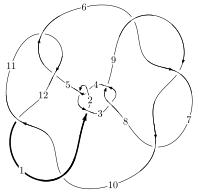
\includegraphics[width=112pt]{../../../GIT/diagram.site/Diagrams/png/917_12a_0116.png}\\
\ \ \ A knot diagram\footnotemark}&
\allowdisplaybreaks
\textbf{Linearized knot diagam} \\
\cline{2-2}
 &
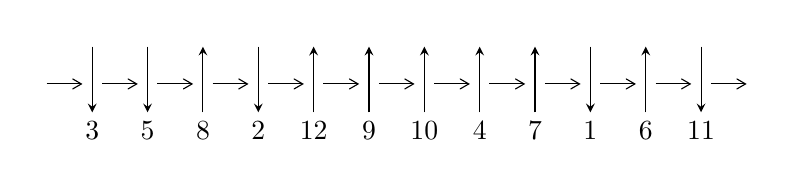
\begin{tikzpicture}[x=20pt, y=17pt]
	% nodes
	\node (C0) at (0, 0) {};
	\node (C1) at (1, 0) {};
	\node (C1U) at (1, +1) {};
	\node (C1D) at (1, -1) {3};

	\node (C2) at (2, 0) {};
	\node (C2U) at (2, +1) {};
	\node (C2D) at (2, -1) {5};

	\node (C3) at (3, 0) {};
	\node (C3U) at (3, +1) {};
	\node (C3D) at (3, -1) {8};

	\node (C4) at (4, 0) {};
	\node (C4U) at (4, +1) {};
	\node (C4D) at (4, -1) {2};

	\node (C5) at (5, 0) {};
	\node (C5U) at (5, +1) {};
	\node (C5D) at (5, -1) {12};

	\node (C6) at (6, 0) {};
	\node (C6U) at (6, +1) {};
	\node (C6D) at (6, -1) {9};

	\node (C7) at (7, 0) {};
	\node (C7U) at (7, +1) {};
	\node (C7D) at (7, -1) {10};

	\node (C8) at (8, 0) {};
	\node (C8U) at (8, +1) {};
	\node (C8D) at (8, -1) {4};

	\node (C9) at (9, 0) {};
	\node (C9U) at (9, +1) {};
	\node (C9D) at (9, -1) {7};

	\node (C10) at (10, 0) {};
	\node (C10U) at (10, +1) {};
	\node (C10D) at (10, -1) {1};

	\node (C11) at (11, 0) {};
	\node (C11U) at (11, +1) {};
	\node (C11D) at (11, -1) {6};

	\node (C12) at (12, 0) {};
	\node (C12U) at (12, +1) {};
	\node (C12D) at (12, -1) {11};
	\node (C13) at (13, 0) {};

	% arrows
	\draw[->,>={angle 60}]
	(C0) edge (C1) (C1) edge (C2) (C2) edge (C3) (C3) edge (C4) (C4) edge (C5) (C5) edge (C6) (C6) edge (C7) (C7) edge (C8) (C8) edge (C9) (C9) edge (C10) (C10) edge (C11) (C11) edge (C12) (C12) edge (C13) ;	\draw[->,>=stealth]
	(C1U) edge (C1D) (C2U) edge (C2D) (C3D) edge (C3U) (C4U) edge (C4D) (C5D) edge (C5U) (C6D) edge (C6U) (C7D) edge (C7U) (C8D) edge (C8U) (C9D) edge (C9U) (C10U) edge (C10D) (C11D) edge (C11U) (C12U) edge (C12D) ;
	\end{tikzpicture} \\
\hhline{~~} \\& 
\textbf{Solving Sequence} \\ \cline{2-2} 
 &
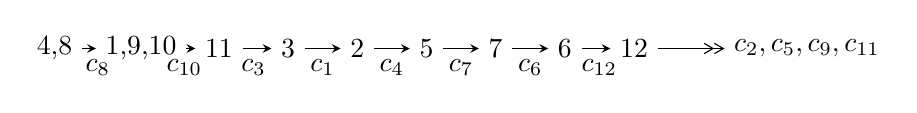
\begin{tikzpicture}[x=25pt, y=7pt]
	% node
	\node (A0) at (-1/8, 0) {4,8};
	\node (A1) at (9/8, 0) {1,9,10};
	\node (A2) at (9/4, 0) {11};
	\node (A3) at (13/4, 0) {3};
	\node (A4) at (17/4, 0) {2};
	\node (A5) at (21/4, 0) {5};
	\node (A6) at (25/4, 0) {7};
	\node (A7) at (29/4, 0) {6};
	\node (A8) at (33/4, 0) {12};
	\node (C1) at (1/2, -1) {$c_{8}$};
	\node (C2) at (7/4, -1) {$c_{10}$};
	\node (C3) at (11/4, -1) {$c_{3}$};
	\node (C4) at (15/4, -1) {$c_{1}$};
	\node (C5) at (19/4, -1) {$c_{4}$};
	\node (C6) at (23/4, -1) {$c_{7}$};
	\node (C7) at (27/4, -1) {$c_{6}$};
	\node (C8) at (31/4, -1) {$c_{12}$};
	\node (A9) at (43/4, 0) {$c_{2},c_{5},c_{9},c_{11}$};

	% edge
	\draw[->,>=stealth]	
	(A0) edge (A1) (A1) edge (A2) (A2) edge (A3) (A3) edge (A4) (A4) edge (A5) (A5) edge (A6) (A6) edge (A7) (A7) edge (A8) ;
	\draw[->>,>={angle 60}]	
	(A8) edge (A9);
\end{tikzpicture} \\ 

\end{tabular} \\

\footnotetext{
The image of knot diagram is generated by the software ``\textbf{Draw programme}" developed by Andrew Bartholomew(\url{http://www.layer8.co.uk/maths/draw/index.htm\#Running-draw}), where we modified some parts for our purpose(\url{https://github.com/CATsTAILs/LinksPainter}).
}\phantom \\ \newline 
\centering \textbf{Ideals for irreducible components\footnotemark of $X_{\text{par}}$} 
 
\begin{align*}
I^u_{1}&=\langle 
4.89741\times10^{143} u^{70}+9.51177\times10^{143} u^{69}+\cdots+1.56737\times10^{147} d+3.91135\times10^{146},\\
\phantom{I^u_{1}}&\phantom{= \langle  }4.81606\times10^{144} u^{70}+8.39188\times10^{144} u^{69}+\cdots+4.38864\times10^{148} c-3.94097\times10^{148},\\
\phantom{I^u_{1}}&\phantom{= \langle  }8.50193\times10^{145} u^{70}+2.17599\times10^{146} u^{69}+\cdots+5.03271\times10^{148} b-4.36186\times10^{148},\\
\phantom{I^u_{1}}&\phantom{= \langle  }-1.70391\times10^{145} u^{70}-5.09324\times10^{145} u^{69}+\cdots+5.03271\times10^{148} a+2.97413\times10^{148},\\
\phantom{I^u_{1}}&\phantom{= \langle  }u^{71}+2 u^{70}+\cdots-1536 u^2+512\rangle \\
I^u_{2}&=\langle 
984 u^8 a^2+450 u^8 a+\cdots+2162 a-142,\;10 u^8 a^2-2340 u^8 a+\cdots+2307 a+6,\\
\phantom{I^u_{2}}&\phantom{= \langle  }379 u^8 a^2+2864 u^8 a+\cdots+2660 a-2336,\;u^8 a+u^8+\cdots- a-1,\\
\phantom{I^u_{2}}&\phantom{= \langle  }u^9- u^8-2 u^7+3 u^6+u^5-3 u^4+2 u^3- u+1\rangle \\
\\
I^v_{1}&=\langle 
c,\;d+1,\;b,\;a- v,\;v^2- v+1\rangle \\
I^v_{2}&=\langle 
a,\;d,\;c-1,\;b- v-1,\;v^2+v+1\rangle \\
I^v_{3}&=\langle 
a,\;d+1,\;c- a,\;b+1,\;v-1\rangle \\
I^v_{4}&=\langle 
c,\;d+1,\;a^2 v^2-2 c a v- v^2 a+c^2+c v+v^2,\;b v+1\rangle \\
\end{align*}
\raggedright * 5 irreducible components of $\dim_{\mathbb{C}}=0$, with total 103 representations.\\
\raggedright * 1 irreducible components of $\dim_{\mathbb{C}}=1$ \\
\footnotetext{All coefficients of polynomials are rational numbers. But the coefficients are sometimes approximated in decimal forms when there is not enough margin.}
\newpage
\renewcommand{\arraystretch}{1}
\centering \section*{I. $I^u_{1}= \langle 4.90\times10^{143} u^{70}+9.51\times10^{143} u^{69}+\cdots+1.57\times10^{147} d+3.91\times10^{146},\;4.82\times10^{144} u^{70}+8.39\times10^{144} u^{69}+\cdots+4.39\times10^{148} c-3.94\times10^{148},\;8.50\times10^{145} u^{70}+2.18\times10^{146} u^{69}+\cdots+5.03\times10^{148} b-4.36\times10^{148},\;-1.70\times10^{145} u^{70}-5.09\times10^{145} u^{69}+\cdots+5.03\times10^{148} a+2.97\times10^{148},\;u^{71}+2 u^{70}+\cdots-1536 u^2+512 \rangle$}
\flushleft \textbf{(i) Arc colorings}\\
\begin{tabular}{m{7pt} m{180pt} m{7pt} m{180pt} }
\flushright $a_{4}=$&$\begin{pmatrix}0\\u\end{pmatrix}$ \\
\flushright $a_{8}=$&$\begin{pmatrix}1\\0\end{pmatrix}$ \\
\flushright $a_{1}=$&$\begin{pmatrix}0.000338567 u^{70}+0.00101203 u^{69}+\cdots-1.54441 u-0.590959\\-0.00168933 u^{70}-0.00432370 u^{69}+\cdots+3.58313 u+0.866702\end{pmatrix}$ \\
\flushright $a_{9}=$&$\begin{pmatrix}1\\- u^2\end{pmatrix}$ \\
\flushright $a_{10}=$&$\begin{pmatrix}-0.000109739 u^{70}-0.000191218 u^{69}+\cdots+0.195370 u+0.897994\\-0.000312460 u^{70}-0.000606862 u^{69}+\cdots+0.402802 u-0.249548\end{pmatrix}$ \\
\flushright $a_{11}=$&$\begin{pmatrix}-0.00183569 u^{70}-0.00101807 u^{69}+\cdots-0.404520 u-0.815831\\0.000206711 u^{70}-0.00283529 u^{69}+\cdots+2.05506 u+2.78231\end{pmatrix}$ \\
\flushright $a_{3}=$&$\begin{pmatrix}- u\\u\end{pmatrix}$ \\
\flushright $a_{2}=$&$\begin{pmatrix}-0.000272969 u^{70}+0.000824654 u^{69}+\cdots-2.23600 u-0.903349\\-0.00107780 u^{70}-0.00413632 u^{69}+\cdots+4.27473 u+1.17909\end{pmatrix}$ \\
\flushright $a_{5}=$&$\begin{pmatrix}0.00135077 u^{70}+0.00331167 u^{69}+\cdots-2.03873 u-0.275743\\-0.00107780 u^{70}-0.00413632 u^{69}+\cdots+4.27473 u+1.17909\end{pmatrix}$ \\
\flushright $a_{7}=$&$\begin{pmatrix}-0.000109739 u^{70}-0.000191218 u^{69}+\cdots+0.195370 u+0.897994\\0.000398397 u^{70}+0.000736742 u^{69}+\cdots-0.458988 u+0.264017\end{pmatrix}$ \\
\flushright $a_{6}=$&$\begin{pmatrix}-0.000422199 u^{70}-0.000798080 u^{69}+\cdots+0.598171 u+0.648446\\0.000578173 u^{70}+0.000945600 u^{69}+\cdots-0.618968 u+0.273263\end{pmatrix}$ \\
\flushright $a_{12}=$&$\begin{pmatrix}-0.00163584 u^{70}-0.00127944 u^{69}+\cdots-0.420031 u-1.00282\\-0.000707113 u^{70}-0.00441555 u^{69}+\cdots+2.78684 u+2.81850\end{pmatrix}$\\&\end{tabular}
\flushleft \textbf{(ii) Obstruction class $= -1$}\\~\\
\flushleft \textbf{(iii) Cusp Shapes $= 0.000644196 u^{70}-0.0111115 u^{69}+\cdots+0.863041 u+15.1191$}\\~\\
\newpage\renewcommand{\arraystretch}{1}
\flushleft \textbf{(iv) u-Polynomials at the component}\newline \\
\begin{tabular}{m{50pt}|m{274pt}}
Crossings & \hspace{64pt}u-Polynomials at each crossing \\
\hline $$\begin{aligned}c_{1}\end{aligned}$$&$\begin{aligned}
&u^{71}+30 u^{70}+\cdots+4640 u+256
\end{aligned}$\\
\hline $$\begin{aligned}c_{2},c_{4}\end{aligned}$$&$\begin{aligned}
&u^{71}-8 u^{70}+\cdots+56 u-16
\end{aligned}$\\
\hline $$\begin{aligned}c_{3},c_{8}\end{aligned}$$&$\begin{aligned}
&u^{71}-2 u^{70}+\cdots+1536 u^2-512
\end{aligned}$\\
\hline $$\begin{aligned}c_{5},c_{11}\end{aligned}$$&$\begin{aligned}
&u^{71}+2 u^{70}+\cdots-5 u^2-4
\end{aligned}$\\
\hline $$\begin{aligned}c_{6},c_{7},c_{9}\end{aligned}$$&$\begin{aligned}
&u^{71}+8 u^{70}+\cdots+56 u-16
\end{aligned}$\\
\hline $$\begin{aligned}c_{10},c_{12}\end{aligned}$$&$\begin{aligned}
&u^{71}+24 u^{70}+\cdots-40 u-16
\end{aligned}$\\
\hline
\end{tabular}\\~\\
\newpage\renewcommand{\arraystretch}{1}
\flushleft \textbf{(v) Riley Polynomials at the component}\newline \\
\begin{tabular}{m{50pt}|m{274pt}}
Crossings & \hspace{64pt}Riley Polynomials at each crossing \\
\hline $$\begin{aligned}c_{1}\end{aligned}$$&$\begin{aligned}
&y^{71}+30 y^{70}+\cdots+5022208 y-65536
\end{aligned}$\\
\hline $$\begin{aligned}c_{2},c_{4}\end{aligned}$$&$\begin{aligned}
&y^{71}-30 y^{70}+\cdots+4640 y-256
\end{aligned}$\\
\hline $$\begin{aligned}c_{3},c_{8}\end{aligned}$$&$\begin{aligned}
&y^{71}-30 y^{70}+\cdots+1572864 y-262144
\end{aligned}$\\
\hline $$\begin{aligned}c_{5},c_{11}\end{aligned}$$&$\begin{aligned}
&y^{71}+24 y^{70}+\cdots-40 y-16
\end{aligned}$\\
\hline $$\begin{aligned}c_{6},c_{7},c_{9}\end{aligned}$$&$\begin{aligned}
&y^{71}-70 y^{70}+\cdots-1504 y-256
\end{aligned}$\\
\hline $$\begin{aligned}c_{10},c_{12}\end{aligned}$$&$\begin{aligned}
&y^{71}+48 y^{70}+\cdots-6880 y-256
\end{aligned}$\\
\hline
\end{tabular}\\~\\
\newpage\flushleft \textbf{(vi) Complex Volumes and Cusp Shapes}
$$\begin{array}{c|c|c}  
\text{Solutions to }I^u_{1}& \I (\text{vol} + \sqrt{-1}CS) & \text{Cusp shape}\\
 \hline 
\begin{aligned}
u &= \phantom{-}0.372595 + 0.922213 I \\
a &= \phantom{-}0.231527 + 0.248876 I \\
b &= \phantom{-}0.846890 - 0.552313 I \\
c &= \phantom{-}0.779729 - 0.752305 I \\
d &= \phantom{-}0.335802 - 0.640838 I\end{aligned}
 & -0.206074 - 1.106620 I & \phantom{-}1.82615 + 2.10157 I \\ \hline\begin{aligned}
u &= \phantom{-}0.372595 - 0.922213 I \\
a &= \phantom{-}0.231527 - 0.248876 I \\
b &= \phantom{-}0.846890 + 0.552313 I \\
c &= \phantom{-}0.779729 + 0.752305 I \\
d &= \phantom{-}0.335802 + 0.640838 I\end{aligned}
 & -0.206074 + 1.106620 I & \phantom{-}1.82615 - 2.10157 I \\ \hline\begin{aligned}
u &= -0.661751 + 0.731261 I \\
a &= -1.22188 + 0.76837 I \\
b &= -0.172678 - 1.098140 I \\
c &= \phantom{-}0.700653 + 0.489800 I \\
d &= \phantom{-}0.041277 + 0.670208 I\end{aligned}
 & -5.31233 + 1.23150 I & -6.16629 - 0.79467 I \\ \hline\begin{aligned}
u &= -0.661751 - 0.731261 I \\
a &= -1.22188 - 0.76837 I \\
b &= -0.172678 + 1.098140 I \\
c &= \phantom{-}0.700653 - 0.489800 I \\
d &= \phantom{-}0.041277 - 0.670208 I\end{aligned}
 & -5.31233 - 1.23150 I & -6.16629 + 0.79467 I \\ \hline\begin{aligned}
u &= -0.216094 + 0.961248 I \\
a &= \phantom{-}0.0234029 - 0.1065430 I \\
b &= -0.945678 - 0.148881 I \\
c &= \phantom{-}0.432999 - 0.019039 I \\
d &= -1.305020 - 0.101353 I\end{aligned}
 & \phantom{-}2.60149 + 2.06138 I & \phantom{-}6.60052 - 3.22142 I \\ \hline\begin{aligned}
u &= -0.216094 - 0.961248 I \\
a &= \phantom{-}0.0234029 + 0.1065430 I \\
b &= -0.945678 + 0.148881 I \\
c &= \phantom{-}0.432999 + 0.019039 I \\
d &= -1.305020 + 0.101353 I\end{aligned}
 & \phantom{-}2.60149 - 2.06138 I & \phantom{-}6.60052 + 3.22142 I\\
 \hline 
 \end{array}$$\newpage$$\begin{array}{c|c|c}  
\text{Solutions to }I^u_{1}& \I (\text{vol} + \sqrt{-1}CS) & \text{Cusp shape}\\
 \hline 
\begin{aligned}
u &= \phantom{-}0.510340 + 0.919175 I \\
a &= \phantom{-}0.422439 + 0.636543 I \\
b &= \phantom{-}0.777623 - 0.912598 I \\
c &= \phantom{-}0.433850 + 0.046431 I \\
d &= -1.278840 + 0.243884 I\end{aligned}
 & -1.22762 - 4.53498 I & -0.48837 + 4.83158 I \\ \hline\begin{aligned}
u &= \phantom{-}0.510340 - 0.919175 I \\
a &= \phantom{-}0.422439 - 0.636543 I \\
b &= \phantom{-}0.777623 + 0.912598 I \\
c &= \phantom{-}0.433850 - 0.046431 I \\
d &= -1.278840 - 0.243884 I\end{aligned}
 & -1.22762 + 4.53498 I & -0.48837 - 4.83158 I \\ \hline\begin{aligned}
u &= -0.843761 + 0.417994 I \\
a &= -2.34521 + 0.64153 I \\
b &= \phantom{-}0.679972 - 0.889234 I \\
c &= \phantom{-}0.642763 + 0.309103 I \\
d &= -0.263568 + 0.607646 I\end{aligned}
 & -1.74336 - 3.95563 I & \phantom{-}0.57229 + 6.63484 I \\ \hline\begin{aligned}
u &= -0.843761 - 0.417994 I \\
a &= -2.34521 - 0.64153 I \\
b &= \phantom{-}0.679972 + 0.889234 I \\
c &= \phantom{-}0.642763 - 0.309103 I \\
d &= -0.263568 - 0.607646 I\end{aligned}
 & -1.74336 + 3.95563 I & \phantom{-}0.57229 - 6.63484 I \\ \hline\begin{aligned}
u &= \phantom{-}0.980094 + 0.401535 I \\
a &= \phantom{-}0.396858 + 0.104153 I \\
b &= -0.149301 - 1.202720 I \\
c &= \phantom{-}0.587267 - 0.304226 I \\
d &= -0.342522 - 0.695475 I\end{aligned}
 & \phantom{-}0.13020 + 4.00402 I & \phantom{-}4.41276 - 6.69495 I \\ \hline\begin{aligned}
u &= \phantom{-}0.980094 - 0.401535 I \\
a &= \phantom{-}0.396858 - 0.104153 I \\
b &= -0.149301 + 1.202720 I \\
c &= \phantom{-}0.587267 + 0.304226 I \\
d &= -0.342522 + 0.695475 I\end{aligned}
 & \phantom{-}0.13020 - 4.00402 I & \phantom{-}4.41276 + 6.69495 I\\
 \hline 
 \end{array}$$\newpage$$\begin{array}{c|c|c}  
\text{Solutions to }I^u_{1}& \I (\text{vol} + \sqrt{-1}CS) & \text{Cusp shape}\\
 \hline 
\begin{aligned}
u &= -0.482781 + 0.984718 I \\
a &= -0.188094 + 0.642789 I \\
b &= -0.975231 - 0.875039 I \\
c &= \phantom{-}0.678408 + 0.703356 I \\
d &= \phantom{-}0.289585 + 0.736539 I\end{aligned}
 & -0.99233 + 6.45679 I & \phantom{-}0.34368 - 6.97496 I \\ \hline\begin{aligned}
u &= -0.482781 - 0.984718 I \\
a &= -0.188094 - 0.642789 I \\
b &= -0.975231 + 0.875039 I \\
c &= \phantom{-}0.678408 - 0.703356 I \\
d &= \phantom{-}0.289585 - 0.736539 I\end{aligned}
 & -0.99233 - 6.45679 I & \phantom{-}0.34368 + 6.97496 I \\ \hline\begin{aligned}
u &= -0.777198 + 0.427799 I \\
a &= -0.190894 + 0.697004 I \\
b &= -0.24801 - 1.87626 I \\
c &= \phantom{-}0.674459 + 0.312849 I \\
d &= -0.220144 + 0.565966 I\end{aligned}
 & -1.94652 + 0.34051 I & -0.37051 + 3.03065 I \\ \hline\begin{aligned}
u &= -0.777198 - 0.427799 I \\
a &= -0.190894 - 0.697004 I \\
b &= -0.24801 + 1.87626 I \\
c &= \phantom{-}0.674459 - 0.312849 I \\
d &= -0.220144 - 0.565966 I\end{aligned}
 & -1.94652 - 0.34051 I & -0.37051 - 3.03065 I \\ \hline\begin{aligned}
u &= -1.127060 + 0.152551 I \\
a &= \phantom{-}0.892844 + 0.350255 I \\
b &= -0.849674 + 0.379750 I \\
c &= -2.51225 - 0.47372 I \\
d &= \phantom{-}1.384380 - 0.072480 I\end{aligned}
 & \phantom{-}4.50468 + 2.47836 I & \phantom{-}7.49354 - 3.38416 I \\ \hline\begin{aligned}
u &= -1.127060 - 0.152551 I \\
a &= \phantom{-}0.892844 - 0.350255 I \\
b &= -0.849674 - 0.379750 I \\
c &= -2.51225 + 0.47372 I \\
d &= \phantom{-}1.384380 + 0.072480 I\end{aligned}
 & \phantom{-}4.50468 - 2.47836 I & \phantom{-}7.49354 + 3.38416 I\\
 \hline 
 \end{array}$$\newpage$$\begin{array}{c|c|c}  
\text{Solutions to }I^u_{1}& \I (\text{vol} + \sqrt{-1}CS) & \text{Cusp shape}\\
 \hline 
\begin{aligned}
u &= -0.982347 + 0.611518 I \\
a &= -1.043830 + 0.376477 I \\
b &= \phantom{-}0.83985 - 1.62811 I \\
c &= \phantom{-}0.577038 + 0.381219 I \\
d &= -0.206434 + 0.797028 I\end{aligned}
 & -4.29573 - 6.37313 I & -3.00781 + 7.19219 I \\ \hline\begin{aligned}
u &= -0.982347 - 0.611518 I \\
a &= -1.043830 - 0.376477 I \\
b &= \phantom{-}0.83985 + 1.62811 I \\
c &= \phantom{-}0.577038 - 0.381219 I \\
d &= -0.206434 - 0.797028 I\end{aligned}
 & -4.29573 + 6.37313 I & -3.00781 - 7.19219 I \\ \hline\begin{aligned}
u &= -1.173990 + 0.222972 I \\
a &= \phantom{-}1.082200 + 0.369743 I \\
b &= -0.979927 + 0.355538 I \\
c &= \phantom{-}0.478067 - 0.168003 I \\
d &= -0.861829 - 0.654286 I\end{aligned}
 & \phantom{-}5.09577 - 1.83902 I & \phantom{-}8.24819 + 0. I\phantom{ +0.000000I} \\ \hline\begin{aligned}
u &= -1.173990 - 0.222972 I \\
a &= \phantom{-}1.082200 - 0.369743 I \\
b &= -0.979927 - 0.355538 I \\
c &= \phantom{-}0.478067 + 0.168003 I \\
d &= -0.861829 + 0.654286 I\end{aligned}
 & \phantom{-}5.09577 + 1.83902 I & \phantom{-}8.24819 + 0. I\phantom{ +0.000000I} \\ \hline\begin{aligned}
u &= \phantom{-}1.203430 + 0.094057 I \\
a &= -0.832154 + 0.565988 I \\
b &= \phantom{-}0.782311 + 0.231668 I \\
c &= \phantom{-}0.487795 + 0.191279 I \\
d &= -0.776824 + 0.696746 I\end{aligned}
 & \phantom{-}5.36659 - 3.89584 I & \phantom{-}8.41567 + 5.55146 I \\ \hline\begin{aligned}
u &= \phantom{-}1.203430 - 0.094057 I \\
a &= -0.832154 - 0.565988 I \\
b &= \phantom{-}0.782311 - 0.231668 I \\
c &= \phantom{-}0.487795 - 0.191279 I \\
d &= -0.776824 - 0.696746 I\end{aligned}
 & \phantom{-}5.36659 + 3.89584 I & \phantom{-}8.41567 - 5.55146 I\\
 \hline 
 \end{array}$$\newpage$$\begin{array}{c|c|c}  
\text{Solutions to }I^u_{1}& \I (\text{vol} + \sqrt{-1}CS) & \text{Cusp shape}\\
 \hline 
\begin{aligned}
u &= -1.117530 + 0.478181 I \\
a &= \phantom{-}1.42291 - 0.12389 I \\
b &= -1.194070 + 0.739062 I \\
c &= -1.92995 - 1.17457 I \\
d &= \phantom{-}1.378100 - 0.230112 I\end{aligned}
 & \phantom{-}3.15531 - 5.12152 I & \phantom{-0.000000 } 0 \\ \hline\begin{aligned}
u &= -1.117530 - 0.478181 I \\
a &= \phantom{-}1.42291 + 0.12389 I \\
b &= -1.194070 - 0.739062 I \\
c &= -1.92995 + 1.17457 I \\
d &= \phantom{-}1.378100 + 0.230112 I\end{aligned}
 & \phantom{-}3.15531 + 5.12152 I & \phantom{-0.000000 } 0 \\ \hline\begin{aligned}
u &= \phantom{-}1.137650 + 0.460214 I \\
a &= \phantom{-}0.741192 - 0.324271 I \\
b &= -0.613390 - 0.807893 I \\
c &= -1.94441 + 1.10888 I \\
d &= \phantom{-}1.388080 + 0.221318 I\end{aligned}
 & \phantom{-}3.19656 + 2.55854 I & \phantom{-0.000000 } 0 \\ \hline\begin{aligned}
u &= \phantom{-}1.137650 - 0.460214 I \\
a &= \phantom{-}0.741192 + 0.324271 I \\
b &= -0.613390 + 0.807893 I \\
c &= -1.94441 - 1.10888 I \\
d &= \phantom{-}1.388080 - 0.221318 I\end{aligned}
 & \phantom{-}3.19656 - 2.55854 I & \phantom{-0.000000 } 0 \\ \hline\begin{aligned}
u &= \phantom{-}0.725491 + 0.260568 I \\
a &= \phantom{-}2.45954 + 0.18676 I \\
b &= -0.615456 - 0.467489 I \\
c &= \phantom{-}0.687076 - 0.223450 I \\
d &= -0.316229 - 0.428062 I\end{aligned}
 & -1.09934 - 1.05821 I & \phantom{-}3.09814 - 1.72718 I \\ \hline\begin{aligned}
u &= \phantom{-}0.725491 - 0.260568 I \\
a &= \phantom{-}2.45954 - 0.18676 I \\
b &= -0.615456 + 0.467489 I \\
c &= \phantom{-}0.687076 + 0.223450 I \\
d &= -0.316229 + 0.428062 I\end{aligned}
 & -1.09934 + 1.05821 I & \phantom{-}3.09814 + 1.72718 I\\
 \hline 
 \end{array}$$\newpage$$\begin{array}{c|c|c}  
\text{Solutions to }I^u_{1}& \I (\text{vol} + \sqrt{-1}CS) & \text{Cusp shape}\\
 \hline 
\begin{aligned}
u &= \phantom{-}0.247645 + 1.226350 I \\
a &= \phantom{-}0.445696 - 1.201150 I \\
b &= -1.18878 + 1.33643 I \\
c &= \phantom{-}0.410272 + 0.019958 I \\
d &= -1.43165 + 0.11829 I\end{aligned}
 & \phantom{-}6.94619 + 1.12108 I & \phantom{-0.000000 } 0 \\ \hline\begin{aligned}
u &= \phantom{-}0.247645 - 1.226350 I \\
a &= \phantom{-}0.445696 + 1.201150 I \\
b &= -1.18878 - 1.33643 I \\
c &= \phantom{-}0.410272 - 0.019958 I \\
d &= -1.43165 - 0.11829 I\end{aligned}
 & \phantom{-}6.94619 - 1.12108 I & \phantom{-0.000000 } 0 \\ \hline\begin{aligned}
u &= -0.464983 + 0.581438 I \\
a &= \phantom{-}0.467028 - 0.609266 I \\
b &= -0.226473 + 0.762464 I \\
c &= \phantom{-}0.469417 - 0.045212 I \\
d &= -1.110720 - 0.203295 I\end{aligned}
 & \phantom{-}1.011140 + 0.938516 I & \phantom{-}3.66296 + 0.79830 I \\ \hline\begin{aligned}
u &= -0.464983 - 0.581438 I \\
a &= \phantom{-}0.467028 + 0.609266 I \\
b &= -0.226473 - 0.762464 I \\
c &= \phantom{-}0.469417 + 0.045212 I \\
d &= -1.110720 + 0.203295 I\end{aligned}
 & \phantom{-}1.011140 - 0.938516 I & \phantom{-}3.66296 - 0.79830 I \\ \hline\begin{aligned}
u &= -0.368570 + 1.210560 I \\
a &= -0.22498 - 1.41639 I \\
b &= \phantom{-}0.91974 + 1.60894 I \\
c &= \phantom{-}0.410382 - 0.029911 I \\
d &= -1.42388 - 0.17667 I\end{aligned}
 & \phantom{-}6.42018 + 4.68044 I & \phantom{-0.000000 } 0 \\ \hline\begin{aligned}
u &= -0.368570 - 1.210560 I \\
a &= -0.22498 + 1.41639 I \\
b &= \phantom{-}0.91974 - 1.60894 I \\
c &= \phantom{-}0.410382 + 0.029911 I \\
d &= -1.42388 + 0.17667 I\end{aligned}
 & \phantom{-}6.42018 - 4.68044 I & \phantom{-0.000000 } 0\\
 \hline 
 \end{array}$$\newpage$$\begin{array}{c|c|c}  
\text{Solutions to }I^u_{1}& \I (\text{vol} + \sqrt{-1}CS) & \text{Cusp shape}\\
 \hline 
\begin{aligned}
u &= \phantom{-}1.248660 + 0.306382 I \\
a &= -1.35825 + 0.40426 I \\
b &= \phantom{-}1.185690 + 0.329456 I \\
c &= -2.03698 + 0.67503 I \\
d &= \phantom{-}1.44235 + 0.14659 I\end{aligned}
 & \phantom{-}7.51654 + 1.91781 I & \phantom{-0.000000 } 0 \\ \hline\begin{aligned}
u &= \phantom{-}1.248660 - 0.306382 I \\
a &= -1.35825 - 0.40426 I \\
b &= \phantom{-}1.185690 - 0.329456 I \\
c &= -2.03698 - 0.67503 I \\
d &= \phantom{-}1.44235 - 0.14659 I\end{aligned}
 & \phantom{-}7.51654 - 1.91781 I & \phantom{-0.000000 } 0 \\ \hline\begin{aligned}
u &= -0.504947 + 1.215580 I \\
a &= \phantom{-}0.553982 + 0.970050 I \\
b &= -1.71071 - 1.04995 I \\
c &= \phantom{-}0.408022 - 0.040917 I \\
d &= -1.42645 - 0.24333 I\end{aligned}
 & \phantom{-}5.42990 + 4.32973 I & \phantom{-0.000000 } 0 \\ \hline\begin{aligned}
u &= -0.504947 - 1.215580 I \\
a &= \phantom{-}0.553982 - 0.970050 I \\
b &= -1.71071 + 1.04995 I \\
c &= \phantom{-}0.408022 + 0.040917 I \\
d &= -1.42645 + 0.24333 I\end{aligned}
 & \phantom{-}5.42990 - 4.32973 I & \phantom{-0.000000 } 0 \\ \hline\begin{aligned}
u &= \phantom{-}1.152900 + 0.667545 I \\
a &= \phantom{-}1.49225 - 0.13001 I \\
b &= -1.39286 - 1.11846 I \\
c &= -1.51029 + 1.23782 I \\
d &= \phantom{-}1.39607 + 0.32462 I\end{aligned}
 & \phantom{-}0.80414 + 10.42400 I & \phantom{-0.000000 } 0 \\ \hline\begin{aligned}
u &= \phantom{-}1.152900 - 0.667545 I \\
a &= \phantom{-}1.49225 + 0.13001 I \\
b &= -1.39286 + 1.11846 I \\
c &= -1.51029 - 1.23782 I \\
d &= \phantom{-}1.39607 - 0.32462 I\end{aligned}
 & \phantom{-}0.80414 - 10.42400 I & \phantom{-0.000000 } 0\\
 \hline 
 \end{array}$$\newpage$$\begin{array}{c|c|c}  
\text{Solutions to }I^u_{1}& \I (\text{vol} + \sqrt{-1}CS) & \text{Cusp shape}\\
 \hline 
\begin{aligned}
u &= \phantom{-}1.185800 + 0.609579 I \\
a &= \phantom{-}1.321700 - 0.330477 I \\
b &= -1.23211 - 0.88467 I \\
c &= \phantom{-}0.512898 - 0.362376 I \\
d &= -0.300514 - 0.918848 I\end{aligned}
 & \phantom{-}2.33908 + 6.73341 I & \phantom{-0.000000 } 0 \\ \hline\begin{aligned}
u &= \phantom{-}1.185800 - 0.609579 I \\
a &= \phantom{-}1.321700 + 0.330477 I \\
b &= -1.23211 + 0.88467 I \\
c &= \phantom{-}0.512898 + 0.362376 I \\
d &= -0.300514 + 0.918848 I\end{aligned}
 & \phantom{-}2.33908 - 6.73341 I & \phantom{-0.000000 } 0 \\ \hline\begin{aligned}
u &= \phantom{-}0.593784 + 1.208600 I \\
a &= -0.434729 + 1.290470 I \\
b &= \phantom{-}1.63973 - 1.36961 I \\
c &= \phantom{-}0.406921 + 0.048241 I \\
d &= -1.42342 + 0.28730 I\end{aligned}
 & \phantom{-}4.48821 - 10.17210 I & \phantom{-0.000000 } 0 \\ \hline\begin{aligned}
u &= \phantom{-}0.593784 - 1.208600 I \\
a &= -0.434729 - 1.290470 I \\
b &= \phantom{-}1.63973 + 1.36961 I \\
c &= \phantom{-}0.406921 - 0.048241 I \\
d &= -1.42342 - 0.28730 I\end{aligned}
 & \phantom{-}4.48821 + 10.17210 I & \phantom{-0.000000 } 0 \\ \hline\begin{aligned}
u &= -1.233000 + 0.545251 I \\
a &= -1.135370 - 0.579184 I \\
b &= \phantom{-}1.066230 - 0.598971 I \\
c &= -1.68270 - 1.01731 I \\
d &= \phantom{-}1.43521 - 0.26312 I\end{aligned}
 & \phantom{-}5.82408 - 7.48275 I & \phantom{-0.000000 } 0 \\ \hline\begin{aligned}
u &= -1.233000 - 0.545251 I \\
a &= -1.135370 + 0.579184 I \\
b &= \phantom{-}1.066230 + 0.598971 I \\
c &= -1.68270 + 1.01731 I \\
d &= \phantom{-}1.43521 + 0.26312 I\end{aligned}
 & \phantom{-}5.82408 + 7.48275 I & \phantom{-0.000000 } 0\\
 \hline 
 \end{array}$$\newpage$$\begin{array}{c|c|c}  
\text{Solutions to }I^u_{1}& \I (\text{vol} + \sqrt{-1}CS) & \text{Cusp shape}\\
 \hline 
\begin{aligned}
u &= \phantom{-}0.176438 + 0.617781 I \\
a &= \phantom{-}0.569269 - 0.700050 I \\
b &= \phantom{-}0.224168 - 0.149459 I \\
c &= \phantom{-}0.464689 + 0.015931 I \\
d &= -1.149450 + 0.073691 I\end{aligned}
 & \phantom{-}0.42738 + 1.60074 I & \phantom{-}0.77404 - 2.18898 I \\ \hline\begin{aligned}
u &= \phantom{-}0.176438 - 0.617781 I \\
a &= \phantom{-}0.569269 + 0.700050 I \\
b &= \phantom{-}0.224168 + 0.149459 I \\
c &= \phantom{-}0.464689 - 0.015931 I \\
d &= -1.149450 - 0.073691 I\end{aligned}
 & \phantom{-}0.42738 - 1.60074 I & \phantom{-}0.77404 + 2.18898 I \\ \hline\begin{aligned}
u &= -1.181300 + 0.680585 I \\
a &= -1.58235 - 0.21766 I \\
b &= \phantom{-}1.49849 - 1.03336 I \\
c &= \phantom{-}0.507502 + 0.382227 I \\
d &= -0.257265 + 0.946913 I\end{aligned}
 & \phantom{-}1.22414 - 12.55690 I & \phantom{-0.000000 } 0 \\ \hline\begin{aligned}
u &= -1.181300 - 0.680585 I \\
a &= -1.58235 + 0.21766 I \\
b &= \phantom{-}1.49849 + 1.03336 I \\
c &= \phantom{-}0.507502 - 0.382227 I \\
d &= -0.257265 - 0.946913 I\end{aligned}
 & \phantom{-}1.22414 + 12.55690 I & \phantom{-0.000000 } 0 \\ \hline\begin{aligned}
u &= -0.010891 + 0.626888 I \\
a &= \phantom{-}0.061320 - 0.678183 I \\
b &= \phantom{-}0.075286 + 0.237093 I \\
c &= \phantom{-}2.55566 - 0.55082 I \\
d &= \phantom{-}0.626081 - 0.080591 I\end{aligned}
 & \phantom{-}0.65592 - 2.35939 I & \phantom{-}1.51759 + 4.85897 I \\ \hline\begin{aligned}
u &= -0.010891 - 0.626888 I \\
a &= \phantom{-}0.061320 + 0.678183 I \\
b &= \phantom{-}0.075286 - 0.237093 I \\
c &= \phantom{-}2.55566 + 0.55082 I \\
d &= \phantom{-}0.626081 + 0.080591 I\end{aligned}
 & \phantom{-}0.65592 + 2.35939 I & \phantom{-}1.51759 - 4.85897 I\\
 \hline 
 \end{array}$$\newpage$$\begin{array}{c|c|c}  
\text{Solutions to }I^u_{1}& \I (\text{vol} + \sqrt{-1}CS) & \text{Cusp shape}\\
 \hline 
\begin{aligned}
u &= \phantom{-}0.617428 + 0.085193 I \\
a &= -0.811434 + 0.311389 I \\
b &= \phantom{-}1.63829 - 0.79430 I \\
c &= \phantom{-}0.704538 - 0.093715 I \\
d &= -0.394694 - 0.185518 I\end{aligned}
 & -0.93328 + 2.67780 I & \phantom{-}3.99337 - 7.95500 I \\ \hline\begin{aligned}
u &= \phantom{-}0.617428 - 0.085193 I \\
a &= -0.811434 - 0.311389 I \\
b &= \phantom{-}1.63829 + 0.79430 I \\
c &= \phantom{-}0.704538 + 0.093715 I \\
d &= -0.394694 + 0.185518 I\end{aligned}
 & -0.93328 - 2.67780 I & \phantom{-}3.99337 + 7.95500 I \\ \hline\begin{aligned}
u &= -0.591164\phantom{ +0.000000I} \\
a &= \phantom{-}0.615382\phantom{ +0.000000I} \\
b &= -0.924859\phantom{ +0.000000I} \\
c &= \phantom{-}0.583091\phantom{ +0.000000I} \\
d &= -0.714998\phantom{ +0.000000I}\end{aligned}
 & \phantom{-}1.02886\phantom{ +0.000000I} & \phantom{-}10.5160\phantom{ +0.000000I} \\ \hline\begin{aligned}
u &= \phantom{-}0.282782 + 0.492299 I \\
a &= \phantom{-}1.18279 - 0.79051 I \\
b &= \phantom{-}0.068443 - 0.284824 I \\
c &= \phantom{-}1.051110 - 0.331574 I \\
d &= \phantom{-}0.134725 - 0.272953 I\end{aligned}
 & -1.67984 - 0.60130 I & -3.90300 + 0.33160 I \\ \hline\begin{aligned}
u &= \phantom{-}0.282782 - 0.492299 I \\
a &= \phantom{-}1.18279 + 0.79051 I \\
b &= \phantom{-}0.068443 + 0.284824 I \\
c &= \phantom{-}1.051110 + 0.331574 I \\
d &= \phantom{-}0.134725 + 0.272953 I\end{aligned}
 & -1.67984 + 0.60130 I & -3.90300 - 0.33160 I \\ \hline\begin{aligned}
u &= \phantom{-}1.33133 + 0.61244 I \\
a &= -2.12188 - 0.10102 I \\
b &= \phantom{-}1.78141 + 0.79853 I \\
c &= -1.50521 + 0.91788 I \\
d &= \phantom{-}1.48428 + 0.29531 I\end{aligned}
 & \phantom{-}10.54930 + 5.35435 I & \phantom{-0.000000 } 0\\
 \hline 
 \end{array}$$\newpage$$\begin{array}{c|c|c}  
\text{Solutions to }I^u_{1}& \I (\text{vol} + \sqrt{-1}CS) & \text{Cusp shape}\\
 \hline 
\begin{aligned}
u &= \phantom{-}1.33133 - 0.61244 I \\
a &= -2.12188 + 0.10102 I \\
b &= \phantom{-}1.78141 - 0.79853 I \\
c &= -1.50521 - 0.91788 I \\
d &= \phantom{-}1.48428 - 0.29531 I\end{aligned}
 & \phantom{-}10.54930 - 5.35435 I & \phantom{-0.000000 } 0 \\ \hline\begin{aligned}
u &= -1.29995 + 0.68416 I \\
a &= \phantom{-}2.14975 - 0.35038 I \\
b &= -1.78132 + 1.02145 I \\
c &= -1.42200 - 1.00239 I \\
d &= \phantom{-}1.46979 - 0.33117 I\end{aligned}
 & \phantom{-}9.4739 - 11.4004 I & \phantom{-0.000000 } 0 \\ \hline\begin{aligned}
u &= -1.29995 - 0.68416 I \\
a &= \phantom{-}2.14975 + 0.35038 I \\
b &= -1.78132 - 1.02145 I \\
c &= -1.42200 + 1.00239 I \\
d &= \phantom{-}1.46979 + 0.33117 I\end{aligned}
 & \phantom{-}9.4739 + 11.4004 I & \phantom{-0.000000 } 0 \\ \hline\begin{aligned}
u &= -1.27239 + 0.75883 I \\
a &= -2.02990 - 0.46254 I \\
b &= \phantom{-}1.99508 - 0.81285 I \\
c &= -1.32486 - 1.06843 I \\
d &= \phantom{-}1.45735 - 0.36883 I\end{aligned}
 & \phantom{-}7.95427 - 11.37060 I & \phantom{-0.000000 } 0 \\ \hline\begin{aligned}
u &= -1.27239 - 0.75883 I \\
a &= -2.02990 + 0.46254 I \\
b &= \phantom{-}1.99508 + 0.81285 I \\
c &= -1.32486 + 1.06843 I \\
d &= \phantom{-}1.45735 + 0.36883 I\end{aligned}
 & \phantom{-}7.95427 + 11.37060 I & \phantom{-0.000000 } 0 \\ \hline\begin{aligned}
u &= \phantom{-}1.24401 + 0.80606 I \\
a &= \phantom{-}2.17907 - 0.26765 I \\
b &= -2.13805 - 1.02984 I \\
c &= -1.26249 + 1.11762 I \\
d &= \phantom{-}1.44408 + 0.39312 I\end{aligned}
 & \phantom{-}6.6365 + 17.3722 I & \phantom{-0.000000 } 0\\
 \hline 
 \end{array}$$\newpage$$\begin{array}{c|c|c}  
\text{Solutions to }I^u_{1}& \I (\text{vol} + \sqrt{-1}CS) & \text{Cusp shape}\\
 \hline 
\begin{aligned}
u &= \phantom{-}1.24401 - 0.80606 I \\
a &= \phantom{-}2.17907 + 0.26765 I \\
b &= -2.13805 + 1.02984 I \\
c &= -1.26249 - 1.11762 I \\
d &= \phantom{-}1.44408 - 0.39312 I\end{aligned}
 & \phantom{-}6.6365 - 17.3722 I & \phantom{-0.000000 } 0 \\ \hline\begin{aligned}
u &= \phantom{-}1.51788 + 0.06429 I \\
a &= -0.63883 - 1.65996 I \\
b &= \phantom{-}0.502635 + 0.680323 I \\
c &= -1.74732 + 0.09337 I \\
d &= \phantom{-}1.57068 + 0.03050 I\end{aligned}
 & \phantom{-}13.78050 + 0.08878 I & \phantom{-0.000000 } 0 \\ \hline\begin{aligned}
u &= \phantom{-}1.51788 - 0.06429 I \\
a &= -0.63883 + 1.65996 I \\
b &= \phantom{-}0.502635 - 0.680323 I \\
c &= -1.74732 - 0.09337 I \\
d &= \phantom{-}1.57068 - 0.03050 I\end{aligned}
 & \phantom{-}13.78050 - 0.08878 I & \phantom{-0.000000 } 0 \\ \hline\begin{aligned}
u &= -1.51414 + 0.16464 I \\
a &= \phantom{-}0.25635 - 1.72702 I \\
b &= -0.145703 + 0.706687 I \\
c &= -1.72459 - 0.23680 I \\
d &= \phantom{-}1.56912 - 0.07814 I\end{aligned}
 & \phantom{-}13.6007 - 6.3599 I & \phantom{-0.000000 } 0 \\ \hline\begin{aligned}
u &= -1.51414 - 0.16464 I \\
a &= \phantom{-}0.25635 + 1.72702 I \\
b &= -0.145703 - 0.706687 I \\
c &= -1.72459 + 0.23680 I \\
d &= \phantom{-}1.56912 + 0.07814 I\end{aligned}
 & \phantom{-}13.6007 + 6.3599 I & \phantom{-0.000000 } 0\\
 \hline 
 \end{array}$$\newpage\newpage\renewcommand{\arraystretch}{1}
\centering \section*{II. $I^u_{2}= \langle 984 a^{2} u^{8}+450 a u^{8}+\cdots+2162 a-142,\;10 a^{2} u^{8}-2340 a u^{8}+\cdots+2307 a+6,\;379 a^{2} u^{8}+2864 a u^{8}+\cdots+2660 a-2336,\;u^8 a+u^8+\cdots- a-1,\;u^9- u^8+\cdots- u+1 \rangle$}
\flushleft \textbf{(i) Arc colorings}\\
\begin{tabular}{m{7pt} m{180pt} m{7pt} m{180pt} }
\flushright $a_{4}=$&$\begin{pmatrix}0\\u\end{pmatrix}$ \\
\flushright $a_{8}=$&$\begin{pmatrix}1\\0\end{pmatrix}$ \\
\flushright $a_{1}=$&$\begin{pmatrix}a\\-0.206991 a^{2} u^{8}-1.56417 a u^{8}+\cdots-1.45276 a+1.27581\end{pmatrix}$ \\
\flushright $a_{9}=$&$\begin{pmatrix}1\\- u^2\end{pmatrix}$ \\
\flushright $a_{10}=$&$\begin{pmatrix}-0.00546150 a^{2} u^{8}+1.27799 a u^{8}+\cdots-1.25997 a-0.00327690\\-0.537411 a^{2} u^{8}-0.245767 a u^{8}+\cdots-1.18078 a+0.0775532\end{pmatrix}$ \\
\flushright $a_{11}=$&$\begin{pmatrix}-0.00546150 a^{2} u^{8}+1.27799 a u^{8}+\cdots-1.25997 a-0.00327690\\-0.436920 a^{2} u^{8}+0.239214 a u^{8}+\cdots-0.797378 a-0.262152\end{pmatrix}$ \\
\flushright $a_{3}=$&$\begin{pmatrix}- u\\u\end{pmatrix}$ \\
\flushright $a_{2}=$&$\begin{pmatrix}0.208629 a^{2} u^{8}+1.18078 a u^{8}+\cdots+1.73075 a-1.07482\\-0.415620 a^{2} u^{8}-2.74495 a u^{8}+\cdots-2.18351 a+2.35063\end{pmatrix}$ \\
\flushright $a_{5}=$&$\begin{pmatrix}0.206991 a^{2} u^{8}+1.56417 a u^{8}+\cdots+0.452758 a-1.27581\\-0.415620 a^{2} u^{8}-2.74495 a u^{8}+\cdots-2.18351 a+2.35063\end{pmatrix}$ \\
\flushright $a_{7}=$&$\begin{pmatrix}-0.00546150 a^{2} u^{8}+1.27799 a u^{8}+\cdots-1.25997 a-0.00327690\\0.637903 a^{2} u^{8}+0.730748 a u^{8}+\cdots+1.56417 a-0.417258\end{pmatrix}$ \\
\flushright $a_{6}=$&$\begin{pmatrix}-0.542873 a^{2} u^{8}+1.03222 a u^{8}+\cdots-2.44074 a+0.0742764\\0.926270 a^{2} u^{8}+1.25287 a u^{8}+\cdots+2.49044 a-1.04424\end{pmatrix}$ \\
\flushright $a_{12}=$&$\begin{pmatrix}-0.171491 a^{2} u^{8}+0.128891 a u^{8}+\cdots-0.762971 a+0.297105\\-0.926270 a^{2} u^{8}-1.25287 a u^{8}+\cdots-2.49044 a+1.04424\end{pmatrix}$\\&\end{tabular}
\flushleft \textbf{(ii) Obstruction class $= -1$}\\~\\
\flushleft \textbf{(iii) Cusp Shapes $= -4 u^7+8 u^5-4 u^4-8 u^3+4 u^2-4 u+2$}\\~\\
\newpage\renewcommand{\arraystretch}{1}
\flushleft \textbf{(iv) u-Polynomials at the component}\newline \\
\begin{tabular}{m{50pt}|m{274pt}}
Crossings & \hspace{64pt}u-Polynomials at each crossing \\
\hline $$\begin{aligned}c_{1}\end{aligned}$$&$\begin{aligned}
&u^{27}+18 u^{26}+\cdots+5 u+1
\end{aligned}$\\
\hline $$\begin{aligned}c_{2},c_{4},c_{6}\\c_{7},c_{9}\end{aligned}$$&$\begin{aligned}
&u^{27}-9 u^{25}+\cdots- u+1
\end{aligned}$\\
\hline $$\begin{aligned}c_{3},c_{8}\end{aligned}$$&$\begin{aligned}
&(u^9+u^8-2 u^7-3 u^6+u^5+3 u^4+2 u^3- u-1)^3
\end{aligned}$\\
\hline $$\begin{aligned}c_{5},c_{11}\end{aligned}$$&$\begin{aligned}
&(u^9+u^8+2 u^7+u^6+3 u^5+u^4+2 u^3+u-1)^3
\end{aligned}$\\
\hline $$\begin{aligned}c_{10},c_{12}\end{aligned}$$&$\begin{aligned}
&(u^9+3 u^8+8 u^7+13 u^6+17 u^5+17 u^4+12 u^3+6 u^2+u-1)^3
\end{aligned}$\\
\hline
\end{tabular}\\~\\
\newpage\renewcommand{\arraystretch}{1}
\flushleft \textbf{(v) Riley Polynomials at the component}\newline \\
\begin{tabular}{m{50pt}|m{274pt}}
Crossings & \hspace{64pt}Riley Polynomials at each crossing \\
\hline $$\begin{aligned}c_{1}\end{aligned}$$&$\begin{aligned}
&y^{27}-18 y^{26}+\cdots-15 y-1
\end{aligned}$\\
\hline $$\begin{aligned}c_{2},c_{4},c_{6}\\c_{7},c_{9}\end{aligned}$$&$\begin{aligned}
&y^{27}-18 y^{26}+\cdots+5 y-1
\end{aligned}$\\
\hline $$\begin{aligned}c_{3},c_{8}\end{aligned}$$&$\begin{aligned}
&(y^9-5 y^8+12 y^7-15 y^6+9 y^5+y^4-4 y^3+2 y^2+y-1)^3
\end{aligned}$\\
\hline $$\begin{aligned}c_{5},c_{11}\end{aligned}$$&$\begin{aligned}
&(y^9+3 y^8+8 y^7+13 y^6+17 y^5+17 y^4+12 y^3+6 y^2+y-1)^3
\end{aligned}$\\
\hline $$\begin{aligned}c_{10},c_{12}\end{aligned}$$&$\begin{aligned}
&(y^9+7 y^8+20 y^7+25 y^6+5 y^5-15 y^4+22 y^2+13 y-1)^3
\end{aligned}$\\
\hline
\end{tabular}\\~\\
\newpage\flushleft \textbf{(vi) Complex Volumes and Cusp Shapes}
$$\begin{array}{c|c|c}  
\text{Solutions to }I^u_{2}& \I (\text{vol} + \sqrt{-1}CS) & \text{Cusp shape}\\
 \hline 
\begin{aligned}
u &= \phantom{-}0.772920 + 0.510351 I \\
a &= -0.875705 - 0.477936 I \\
b &= \phantom{-}0.681130 + 0.860855 I \\
c &= \phantom{-}0.675016 - 0.354446 I \\
d &= -0.161261 - 0.609769 I\end{aligned}
 & -1.78344 + 2.09337 I & -0.51499 - 4.16283 I \\ \hline\begin{aligned}
u &= \phantom{-}0.772920 + 0.510351 I \\
a &= \phantom{-}0.410374 + 0.842624 I \\
b &= -0.01297 - 2.10540 I \\
c &= \phantom{-}0.473784 + 0.085898 I \\
d &= -1.043500 + 0.370490 I\end{aligned}
 & -1.78344 + 2.09337 I & -0.51499 - 4.16283 I \\ \hline\begin{aligned}
u &= \phantom{-}0.772920 + 0.510351 I \\
a &= \phantom{-}2.01117 + 0.65601 I \\
b &= -0.412038 - 0.965972 I \\
c &= -2.06450 + 2.41256 I \\
d &= \phantom{-}1.204760 + 0.239279 I\end{aligned}
 & -1.78344 + 2.09337 I & -0.51499 - 4.16283 I \\ \hline\begin{aligned}
u &= \phantom{-}0.772920 - 0.510351 I \\
a &= -0.875705 + 0.477936 I \\
b &= \phantom{-}0.681130 - 0.860855 I \\
c &= \phantom{-}0.675016 + 0.354446 I \\
d &= -0.161261 + 0.609769 I\end{aligned}
 & -1.78344 - 2.09337 I & -0.51499 + 4.16283 I \\ \hline\begin{aligned}
u &= \phantom{-}0.772920 - 0.510351 I \\
a &= \phantom{-}0.410374 - 0.842624 I \\
b &= -0.01297 + 2.10540 I \\
c &= \phantom{-}0.473784 - 0.085898 I \\
d &= -1.043500 - 0.370490 I\end{aligned}
 & -1.78344 - 2.09337 I & -0.51499 + 4.16283 I \\ \hline\begin{aligned}
u &= \phantom{-}0.772920 - 0.510351 I \\
a &= \phantom{-}2.01117 - 0.65601 I \\
b &= -0.412038 + 0.965972 I \\
c &= -2.06450 - 2.41256 I \\
d &= \phantom{-}1.204760 - 0.239279 I\end{aligned}
 & -1.78344 - 2.09337 I & -0.51499 + 4.16283 I\\
 \hline 
 \end{array}$$\newpage$$\begin{array}{c|c|c}  
\text{Solutions to }I^u_{2}& \I (\text{vol} + \sqrt{-1}CS) & \text{Cusp shape}\\
 \hline 
\begin{aligned}
u &= -0.825933\phantom{ +0.000000I} \\
a &= \phantom{-}0.566697 + 0.073493 I \\
b &= -0.840182 - 0.678317 I \\
c &= \phantom{-}0.580888 - 0.143767 I \\
d &= -0.622141 - 0.401472 I\end{aligned}
 & \phantom{-}1.19845\phantom{ +0.000000I} & \phantom{-}8.65230\phantom{ +0.000000I} \\ \hline\begin{aligned}
u &= -0.825933\phantom{ +0.000000I} \\
a &= \phantom{-}0.566697 - 0.073493 I \\
b &= -0.840182 + 0.678317 I \\
c &= \phantom{-}0.580888 + 0.143767 I \\
d &= -0.622141 + 0.401472 I\end{aligned}
 & \phantom{-}1.19845\phantom{ +0.000000I} & \phantom{-}8.65230\phantom{ +0.000000I} \\ \hline\begin{aligned}
u &= -0.825933\phantom{ +0.000000I} \\
a &= -2.78526\phantom{ +0.000000I} \\
b &= \phantom{-}0.910725\phantom{ +0.000000I} \\
c &= -4.09362\phantom{ +0.000000I} \\
d &= \phantom{-}1.24428\phantom{ +0.000000I}\end{aligned}
 & \phantom{-}1.19845\phantom{ +0.000000I} & \phantom{-}8.65230\phantom{ +0.000000I} \\ \hline\begin{aligned}
u &= -1.173910 + 0.391555 I \\
a &= -0.542704 - 0.501634 I \\
b &= \phantom{-}0.438594 - 0.586599 I \\
c &= \phantom{-}0.459000 - 0.147401 I \\
d &= -0.974973 - 0.634235 I\end{aligned}
 & \phantom{-}4.37135 - 1.33617 I & \phantom{-}7.28409 + 0.70175 I \\ \hline\begin{aligned}
u &= -1.173910 + 0.391555 I \\
a &= \phantom{-}1.393210 + 0.120134 I \\
b &= -1.198840 + 0.548367 I \\
c &= \phantom{-}0.525422 + 0.301815 I \\
d &= -0.431041 + 0.822025 I\end{aligned}
 & \phantom{-}4.37135 - 1.33617 I & \phantom{-}7.28409 + 0.70175 I \\ \hline\begin{aligned}
u &= -1.173910 + 0.391555 I \\
a &= -3.19833 + 1.16461 I \\
b &= \phantom{-}1.57493 - 1.25625 I \\
c &= -2.02893 - 0.93842 I \\
d &= \phantom{-}1.40601 - 0.18779 I\end{aligned}
 & \phantom{-}4.37135 - 1.33617 I & \phantom{-}7.28409 + 0.70175 I\\
 \hline 
 \end{array}$$\newpage$$\begin{array}{c|c|c}  
\text{Solutions to }I^u_{2}& \I (\text{vol} + \sqrt{-1}CS) & \text{Cusp shape}\\
 \hline 
\begin{aligned}
u &= -1.173910 - 0.391555 I \\
a &= -0.542704 + 0.501634 I \\
b &= \phantom{-}0.438594 + 0.586599 I \\
c &= \phantom{-}0.459000 + 0.147401 I \\
d &= -0.974973 + 0.634235 I\end{aligned}
 & \phantom{-}4.37135 + 1.33617 I & \phantom{-}7.28409 - 0.70175 I \\ \hline\begin{aligned}
u &= -1.173910 - 0.391555 I \\
a &= \phantom{-}1.393210 - 0.120134 I \\
b &= -1.198840 - 0.548367 I \\
c &= \phantom{-}0.525422 - 0.301815 I \\
d &= -0.431041 - 0.822025 I\end{aligned}
 & \phantom{-}4.37135 + 1.33617 I & \phantom{-}7.28409 - 0.70175 I \\ \hline\begin{aligned}
u &= -1.173910 - 0.391555 I \\
a &= -3.19833 - 1.16461 I \\
b &= \phantom{-}1.57493 + 1.25625 I \\
c &= -2.02893 + 0.93842 I \\
d &= \phantom{-}1.40601 + 0.18779 I\end{aligned}
 & \phantom{-}4.37135 + 1.33617 I & \phantom{-}7.28409 - 0.70175 I \\ \hline\begin{aligned}
u &= \phantom{-}0.141484 + 0.739668 I \\
a &= -0.127412 - 0.662482 I \\
b &= -0.274121 + 0.513437 I \\
c &= \phantom{-}1.24382 - 0.80550 I \\
d &= \phantom{-}0.433577 - 0.366819 I\end{aligned}
 & \phantom{-}0.61694 - 2.45442 I & \phantom{-}2.32792 + 2.91298 I \\ \hline\begin{aligned}
u &= \phantom{-}0.141484 + 0.739668 I \\
a &= \phantom{-}0.313138 - 0.492021 I \\
b &= \phantom{-}0.423223 - 0.044379 I \\
c &= \phantom{-}1.58042 + 2.09413 I \\
d &= \phantom{-}0.770392 + 0.304242 I\end{aligned}
 & \phantom{-}0.61694 - 2.45442 I & \phantom{-}2.32792 + 2.91298 I \\ \hline\begin{aligned}
u &= \phantom{-}0.141484 + 0.739668 I \\
a &= \phantom{-}0.09724 + 2.63384 I \\
b &= \phantom{-}0.06688 - 4.55687 I \\
c &= \phantom{-}0.453361 + 0.012872 I \\
d &= -1.203970 + 0.062577 I\end{aligned}
 & \phantom{-}0.61694 - 2.45442 I & \phantom{-}2.32792 + 2.91298 I\\
 \hline 
 \end{array}$$\newpage$$\begin{array}{c|c|c}  
\text{Solutions to }I^u_{2}& \I (\text{vol} + \sqrt{-1}CS) & \text{Cusp shape}\\
 \hline 
\begin{aligned}
u &= \phantom{-}0.141484 - 0.739668 I \\
a &= -0.127412 + 0.662482 I \\
b &= -0.274121 - 0.513437 I \\
c &= \phantom{-}1.24382 + 0.80550 I \\
d &= \phantom{-}0.433577 + 0.366819 I\end{aligned}
 & \phantom{-}0.61694 + 2.45442 I & \phantom{-}2.32792 - 2.91298 I \\ \hline\begin{aligned}
u &= \phantom{-}0.141484 - 0.739668 I \\
a &= \phantom{-}0.313138 + 0.492021 I \\
b &= \phantom{-}0.423223 + 0.044379 I \\
c &= \phantom{-}1.58042 - 2.09413 I \\
d &= \phantom{-}0.770392 - 0.304242 I\end{aligned}
 & \phantom{-}0.61694 + 2.45442 I & \phantom{-}2.32792 - 2.91298 I \\ \hline\begin{aligned}
u &= \phantom{-}0.141484 - 0.739668 I \\
a &= \phantom{-}0.09724 - 2.63384 I \\
b &= \phantom{-}0.06688 + 4.55687 I \\
c &= \phantom{-}0.453361 - 0.012872 I \\
d &= -1.203970 - 0.062577 I\end{aligned}
 & \phantom{-}0.61694 + 2.45442 I & \phantom{-}2.32792 - 2.91298 I \\ \hline\begin{aligned}
u &= \phantom{-}1.172470 + 0.500383 I \\
a &= \phantom{-}0.912481 - 0.404680 I \\
b &= -0.807640 - 0.750845 I \\
c &= \phantom{-}0.447551 + 0.136556 I \\
d &= -1.044080 + 0.623685 I\end{aligned}
 & \phantom{-}3.59813 + 7.08493 I & \phantom{-}5.57680 - 5.91335 I \\ \hline\begin{aligned}
u &= \phantom{-}1.172470 + 0.500383 I \\
a &= -1.56344 - 0.08945 I \\
b &= \phantom{-}1.31021 + 0.73026 I \\
c &= \phantom{-}0.523388 - 0.332558 I \\
d &= -0.361113 - 0.864843 I\end{aligned}
 & \phantom{-}3.59813 + 7.08493 I & \phantom{-}5.57680 - 5.91335 I \\ \hline\begin{aligned}
u &= \phantom{-}1.172470 + 0.500383 I \\
a &= \phantom{-}2.99591 + 1.49490 I \\
b &= -1.40454 - 1.59601 I \\
c &= -1.82241 + 1.08463 I \\
d &= \phantom{-}1.40520 + 0.24116 I\end{aligned}
 & \phantom{-}3.59813 + 7.08493 I & \phantom{-}5.57680 - 5.91335 I\\
 \hline 
 \end{array}$$\newpage$$\begin{array}{c|c|c}  
\text{Solutions to }I^u_{2}& \I (\text{vol} + \sqrt{-1}CS) & \text{Cusp shape}\\
 \hline 
\begin{aligned}
u &= \phantom{-}1.172470 - 0.500383 I \\
a &= \phantom{-}0.912481 + 0.404680 I \\
b &= -0.807640 + 0.750845 I \\
c &= \phantom{-}0.447551 - 0.136556 I \\
d &= -1.044080 - 0.623685 I\end{aligned}
 & \phantom{-}3.59813 - 7.08493 I & \phantom{-}5.57680 + 5.91335 I \\ \hline\begin{aligned}
u &= \phantom{-}1.172470 - 0.500383 I \\
a &= -1.56344 + 0.08945 I \\
b &= \phantom{-}1.31021 - 0.73026 I \\
c &= \phantom{-}0.523388 + 0.332558 I \\
d &= -0.361113 + 0.864843 I\end{aligned}
 & \phantom{-}3.59813 - 7.08493 I & \phantom{-}5.57680 + 5.91335 I \\ \hline\begin{aligned}
u &= \phantom{-}1.172470 - 0.500383 I \\
a &= \phantom{-}2.99591 - 1.49490 I \\
b &= -1.40454 + 1.59601 I \\
c &= -1.82241 - 1.08463 I \\
d &= \phantom{-}1.40520 - 0.24116 I\end{aligned}
 & \phantom{-}3.59813 - 7.08493 I & \phantom{-}5.57680 + 5.91335 I\\
 \hline 
 \end{array}$$\newpage\newpage\renewcommand{\arraystretch}{1}
\centering \section*{III. $I^v_{1}= \langle c,\;d+1,\;b,\;a- v,\;v^2- v+1 \rangle$}
\flushleft \textbf{(i) Arc colorings}\\
\begin{tabular}{m{7pt} m{180pt} m{7pt} m{180pt} }
\flushright $a_{4}=$&$\begin{pmatrix}v\\0\end{pmatrix}$ \\
\flushright $a_{8}=$&$\begin{pmatrix}1\\0\end{pmatrix}$ \\
\flushright $a_{1}=$&$\begin{pmatrix}v\\0\end{pmatrix}$ \\
\flushright $a_{9}=$&$\begin{pmatrix}1\\0\end{pmatrix}$ \\
\flushright $a_{10}=$&$\begin{pmatrix}0\\-1\end{pmatrix}$ \\
\flushright $a_{11}=$&$\begin{pmatrix}v-1\\-1\end{pmatrix}$ \\
\flushright $a_{3}=$&$\begin{pmatrix}v\\0\end{pmatrix}$ \\
\flushright $a_{2}=$&$\begin{pmatrix}v\\0\end{pmatrix}$ \\
\flushright $a_{5}=$&$\begin{pmatrix}v\\0\end{pmatrix}$ \\
\flushright $a_{7}=$&$\begin{pmatrix}1\\1\end{pmatrix}$ \\
\flushright $a_{6}=$&$\begin{pmatrix}0\\1\end{pmatrix}$ \\
\flushright $a_{12}=$&$\begin{pmatrix}v-1\\- v\end{pmatrix}$\\&\end{tabular}
\flushleft \textbf{(ii) Obstruction class $= 1$}\\~\\
\flushleft \textbf{(iii) Cusp Shapes $= 4 v+7$}\\~\\
\newpage\renewcommand{\arraystretch}{1}
\flushleft \textbf{(iv) u-Polynomials at the component}\newline \\
\begin{tabular}{m{50pt}|m{274pt}}
Crossings & \hspace{64pt}u-Polynomials at each crossing \\
\hline $$\begin{aligned}c_{1},c_{2},c_{3}\\c_{4},c_{8}\end{aligned}$$&$\begin{aligned}
&u^2
\end{aligned}$\\
\hline $$\begin{aligned}c_{5},c_{10}\end{aligned}$$&$\begin{aligned}
&u^2- u+1
\end{aligned}$\\
\hline $$\begin{aligned}c_{6},c_{7}\end{aligned}$$&$\begin{aligned}
&(u+1)^2
\end{aligned}$\\
\hline $$\begin{aligned}c_{9}\end{aligned}$$&$\begin{aligned}
&(u-1)^2
\end{aligned}$\\
\hline $$\begin{aligned}c_{11},c_{12}\end{aligned}$$&$\begin{aligned}
&u^2+u+1
\end{aligned}$\\
\hline
\end{tabular}\\~\\
\newpage\renewcommand{\arraystretch}{1}
\flushleft \textbf{(v) Riley Polynomials at the component}\newline \\
\begin{tabular}{m{50pt}|m{274pt}}
Crossings & \hspace{64pt}Riley Polynomials at each crossing \\
\hline $$\begin{aligned}c_{1},c_{2},c_{3}\\c_{4},c_{8}\end{aligned}$$&$\begin{aligned}
&y^2
\end{aligned}$\\
\hline $$\begin{aligned}c_{5},c_{10},c_{11}\\c_{12}\end{aligned}$$&$\begin{aligned}
&y^2+y+1
\end{aligned}$\\
\hline $$\begin{aligned}c_{6},c_{7},c_{9}\end{aligned}$$&$\begin{aligned}
&(y-1)^2
\end{aligned}$\\
\hline
\end{tabular}\\~\\
\newpage\flushleft \textbf{(vi) Complex Volumes and Cusp Shapes}
$$\begin{array}{c|c|c}  
\text{Solutions to }I^v_{1}& \I (\text{vol} + \sqrt{-1}CS) & \text{Cusp shape}\\
 \hline 
\begin{aligned}
v &= \phantom{-}0.500000 + 0.866025 I \\
a &= \phantom{-}0.500000 + 0.866025 I \\
b &= \phantom{-0.000000 } 0 \\
c &= \phantom{-0.000000 } 0 \\
d &= -1.00000\phantom{ +0.000000I}\end{aligned}
 & \phantom{-}1.64493 - 2.02988 I & \phantom{-}9.00000 + 3.46410 I \\ \hline\begin{aligned}
v &= \phantom{-}0.500000 - 0.866025 I \\
a &= \phantom{-}0.500000 - 0.866025 I \\
b &= \phantom{-0.000000 } 0 \\
c &= \phantom{-0.000000 } 0 \\
d &= -1.00000\phantom{ +0.000000I}\end{aligned}
 & \phantom{-}1.64493 + 2.02988 I & \phantom{-}9.00000 - 3.46410 I\\
 \hline 
 \end{array}$$\newpage\newpage\renewcommand{\arraystretch}{1}
\centering \section*{IV. $I^v_{2}= \langle a,\;d,\;c-1,\;b- v-1,\;v^2+v+1 \rangle$}
\flushleft \textbf{(i) Arc colorings}\\
\begin{tabular}{m{7pt} m{180pt} m{7pt} m{180pt} }
\flushright $a_{4}=$&$\begin{pmatrix}v\\0\end{pmatrix}$ \\
\flushright $a_{8}=$&$\begin{pmatrix}1\\0\end{pmatrix}$ \\
\flushright $a_{1}=$&$\begin{pmatrix}0\\v+1\end{pmatrix}$ \\
\flushright $a_{9}=$&$\begin{pmatrix}1\\0\end{pmatrix}$ \\
\flushright $a_{10}=$&$\begin{pmatrix}1\\0\end{pmatrix}$ \\
\flushright $a_{11}=$&$\begin{pmatrix}1\\v\end{pmatrix}$ \\
\flushright $a_{3}=$&$\begin{pmatrix}v\\0\end{pmatrix}$ \\
\flushright $a_{2}=$&$\begin{pmatrix}v\\v+1\end{pmatrix}$ \\
\flushright $a_{5}=$&$\begin{pmatrix}0\\- v-1\end{pmatrix}$ \\
\flushright $a_{7}=$&$\begin{pmatrix}1\\0\end{pmatrix}$ \\
\flushright $a_{6}=$&$\begin{pmatrix}1\\0\end{pmatrix}$ \\
\flushright $a_{12}=$&$\begin{pmatrix}v+1\\v\end{pmatrix}$\\&\end{tabular}
\flushleft \textbf{(ii) Obstruction class $= 1$}\\~\\
\flushleft \textbf{(iii) Cusp Shapes $= 4 v-1$}\\~\\
\newpage\renewcommand{\arraystretch}{1}
\flushleft \textbf{(iv) u-Polynomials at the component}\newline \\
\begin{tabular}{m{50pt}|m{274pt}}
Crossings & \hspace{64pt}u-Polynomials at each crossing \\
\hline $$\begin{aligned}c_{1},c_{2}\end{aligned}$$&$\begin{aligned}
&(u-1)^2
\end{aligned}$\\
\hline $$\begin{aligned}c_{3},c_{6},c_{7}\\c_{8},c_{9}\end{aligned}$$&$\begin{aligned}
&u^2
\end{aligned}$\\
\hline $$\begin{aligned}c_{4}\end{aligned}$$&$\begin{aligned}
&(u+1)^2
\end{aligned}$\\
\hline $$\begin{aligned}c_{5},c_{12}\end{aligned}$$&$\begin{aligned}
&u^2+u+1
\end{aligned}$\\
\hline $$\begin{aligned}c_{10},c_{11}\end{aligned}$$&$\begin{aligned}
&u^2- u+1
\end{aligned}$\\
\hline
\end{tabular}\\~\\
\newpage\renewcommand{\arraystretch}{1}
\flushleft \textbf{(v) Riley Polynomials at the component}\newline \\
\begin{tabular}{m{50pt}|m{274pt}}
Crossings & \hspace{64pt}Riley Polynomials at each crossing \\
\hline $$\begin{aligned}c_{1},c_{2},c_{4}\end{aligned}$$&$\begin{aligned}
&(y-1)^2
\end{aligned}$\\
\hline $$\begin{aligned}c_{3},c_{6},c_{7}\\c_{8},c_{9}\end{aligned}$$&$\begin{aligned}
&y^2
\end{aligned}$\\
\hline $$\begin{aligned}c_{5},c_{10},c_{11}\\c_{12}\end{aligned}$$&$\begin{aligned}
&y^2+y+1
\end{aligned}$\\
\hline
\end{tabular}\\~\\
\newpage\flushleft \textbf{(vi) Complex Volumes and Cusp Shapes}
$$\begin{array}{c|c|c}  
\text{Solutions to }I^v_{2}& \I (\text{vol} + \sqrt{-1}CS) & \text{Cusp shape}\\
 \hline 
\begin{aligned}
v &= -0.500000 + 0.866025 I \\
a &= \phantom{-0.000000 } 0 \\
b &= \phantom{-}0.500000 + 0.866025 I \\
c &= \phantom{-}1.00000\phantom{ +0.000000I} \\
d &= \phantom{-0.000000 } 0\end{aligned}
 & -1.64493 - 2.02988 I & -3.00000 + 3.46410 I \\ \hline\begin{aligned}
v &= -0.500000 - 0.866025 I \\
a &= \phantom{-0.000000 } 0 \\
b &= \phantom{-}0.500000 - 0.866025 I \\
c &= \phantom{-}1.00000\phantom{ +0.000000I} \\
d &= \phantom{-0.000000 } 0\end{aligned}
 & -1.64493 + 2.02988 I & -3.00000 - 3.46410 I\\
 \hline 
 \end{array}$$\newpage\newpage\renewcommand{\arraystretch}{1}
\centering \section*{V. $I^v_{3}= \langle a,\;d+1,\;c- a,\;b+1,\;v-1 \rangle$}
\flushleft \textbf{(i) Arc colorings}\\
\begin{tabular}{m{7pt} m{180pt} m{7pt} m{180pt} }
\flushright $a_{4}=$&$\begin{pmatrix}1\\0\end{pmatrix}$ \\
\flushright $a_{8}=$&$\begin{pmatrix}1\\0\end{pmatrix}$ \\
\flushright $a_{1}=$&$\begin{pmatrix}0\\-1\end{pmatrix}$ \\
\flushright $a_{9}=$&$\begin{pmatrix}1\\0\end{pmatrix}$ \\
\flushright $a_{10}=$&$\begin{pmatrix}0\\-1\end{pmatrix}$ \\
\flushright $a_{11}=$&$\begin{pmatrix}0\\-1\end{pmatrix}$ \\
\flushright $a_{3}=$&$\begin{pmatrix}1\\0\end{pmatrix}$ \\
\flushright $a_{2}=$&$\begin{pmatrix}1\\-1\end{pmatrix}$ \\
\flushright $a_{5}=$&$\begin{pmatrix}0\\1\end{pmatrix}$ \\
\flushright $a_{7}=$&$\begin{pmatrix}1\\1\end{pmatrix}$ \\
\flushright $a_{6}=$&$\begin{pmatrix}0\\1\end{pmatrix}$ \\
\flushright $a_{12}=$&$\begin{pmatrix}0\\-1\end{pmatrix}$\\&\end{tabular}
\flushleft \textbf{(ii) Obstruction class $= 1$}\\~\\
\flushleft \textbf{(iii) Cusp Shapes $= 0$}\\~\\
\newpage\renewcommand{\arraystretch}{1}
\flushleft \textbf{(iv) u-Polynomials at the component}\newline \\
\begin{tabular}{m{50pt}|m{274pt}}
Crossings & \hspace{64pt}u-Polynomials at each crossing \\
\hline $$\begin{aligned}c_{1},c_{2},c_{9}\end{aligned}$$&$\begin{aligned}
&u-1
\end{aligned}$\\
\hline $$\begin{aligned}c_{3},c_{5},c_{8}\\c_{10},c_{11},c_{12}\end{aligned}$$&$\begin{aligned}
&u
\end{aligned}$\\
\hline $$\begin{aligned}c_{4},c_{6},c_{7}\end{aligned}$$&$\begin{aligned}
&u+1
\end{aligned}$\\
\hline
\end{tabular}\\~\\
\newpage\renewcommand{\arraystretch}{1}
\flushleft \textbf{(v) Riley Polynomials at the component}\newline \\
\begin{tabular}{m{50pt}|m{274pt}}
Crossings & \hspace{64pt}Riley Polynomials at each crossing \\
\hline $$\begin{aligned}c_{1},c_{2},c_{4}\\c_{6},c_{7},c_{9}\end{aligned}$$&$\begin{aligned}
&y-1
\end{aligned}$\\
\hline $$\begin{aligned}c_{3},c_{5},c_{8}\\c_{10},c_{11},c_{12}\end{aligned}$$&$\begin{aligned}
&y
\end{aligned}$\\
\hline
\end{tabular}\\~\\
\newpage\flushleft \textbf{(vi) Complex Volumes and Cusp Shapes}
$$\begin{array}{c|c|c}  
\text{Solutions to }I^v_{3}& \I (\text{vol} + \sqrt{-1}CS) & \text{Cusp shape}\\
 \hline 
\begin{aligned}
v &= \phantom{-}1.00000\phantom{ +0.000000I} \\
a &= \phantom{-0.000000 } 0 \\
b &= -1.00000\phantom{ +0.000000I} \\
c &= \phantom{-0.000000 } 0 \\
d &= -1.00000\phantom{ +0.000000I}\end{aligned}
 & \phantom{-0.000000 } 0 & \phantom{-0.000000 } 0\\
 \hline 
 \end{array}$$\newpage\newpage\renewcommand{\arraystretch}{1}
\centering \section*{VI. $I^v_{4}= \langle c,\;d+1,\;a^2 v^2-2 c a v- v^2 a+c^2+c v+v^2,\;b v+1 \rangle$}
\flushleft \textbf{(i) Arc colorings}\\
\begin{tabular}{m{7pt} m{180pt} m{7pt} m{180pt} }
\flushright $a_{4}=$&$\begin{pmatrix}v\\0\end{pmatrix}$ \\
\flushright $a_{8}=$&$\begin{pmatrix}1\\0\end{pmatrix}$ \\
\flushright $a_{1}=$&$\begin{pmatrix}a\\b\end{pmatrix}$ \\
\flushright $a_{9}=$&$\begin{pmatrix}1\\0\end{pmatrix}$ \\
\flushright $a_{10}=$&$\begin{pmatrix}0\\-1\end{pmatrix}$ \\
\flushright $a_{11}=$&$\begin{pmatrix}a-1\\b a-1\end{pmatrix}$ \\
\flushright $a_{3}=$&$\begin{pmatrix}v\\0\end{pmatrix}$ \\
\flushright $a_{2}=$&$\begin{pmatrix}a+v\\b\end{pmatrix}$ \\
\flushright $a_{5}=$&$\begin{pmatrix}- a\\- b\end{pmatrix}$ \\
\flushright $a_{7}=$&$\begin{pmatrix}1\\1\end{pmatrix}$ \\
\flushright $a_{6}=$&$\begin{pmatrix}0\\1\end{pmatrix}$ \\
\flushright $a_{12}=$&$\begin{pmatrix}a-1\\b a- a\end{pmatrix}$\\&\end{tabular}
\flushleft \textbf{(ii) Obstruction class $= -1$}\\~\\
\flushleft \textbf{(iii) Cusp Shapes $= - b^2- v^2+4 a$}\\~\\
\flushleft \textbf{(iv) u-Polynomials at the component} : It cannot be defined for a positive dimension component.\\~\\
\flushleft \textbf{(v) Riley Polynomials at the component} : It cannot be defined for a positive dimension component.\\~\\
\newpage\flushleft \textbf{(iv) Complex Volumes and Cusp Shapes}
$$\begin{array}{c|c|c} 
\text{Solution to }I^v_{4}& \I (\text{vol} + \sqrt{-1}CS) & \text{Cusp shape}\\
 \hline 
\begin{aligned}
v &= \cdots \\
a &= \cdots \\
b &= \cdots \\
c &= \cdots \\
d &= \cdots\end{aligned}
 & \phantom{-0.000000 -}2.02988 I & \phantom{-}4.09661 + 3.75064 I\\
 \hline 
 \end{array}
$$
\newpage\renewcommand{\arraystretch}{1}
\centering \section*{ VII. u-Polynomials}
\begin{tabular}{m{50pt}|m{274pt}}
Crossings & \hspace{64pt}u-Polynomials at each crossing \\
\hline $$\begin{aligned}c_{1}\end{aligned}$$&$\begin{aligned}
&u^2(u-1)^3(u^{27}+18 u^{26}+\cdots+5 u+1)\\
&\cdot(u^{71}+30 u^{70}+\cdots+4640 u+256)
\end{aligned}$\\
\hline $$\begin{aligned}c_{2}\end{aligned}$$&$\begin{aligned}
&u^2(u-1)^3(u^{27}-9 u^{25}+\cdots- u+1)(u^{71}-8 u^{70}+\cdots+56 u-16)
\end{aligned}$\\
\hline $$\begin{aligned}c_{3},c_{8}\end{aligned}$$&$\begin{aligned}
&u^5(u^9+u^8-2 u^7-3 u^6+u^5+3 u^4+2 u^3- u-1)^3\\
&\cdot(u^{71}-2 u^{70}+\cdots+1536 u^2-512)
\end{aligned}$\\
\hline $$\begin{aligned}c_{4}\end{aligned}$$&$\begin{aligned}
&u^2(u+1)^3(u^{27}-9 u^{25}+\cdots- u+1)(u^{71}-8 u^{70}+\cdots+56 u-16)
\end{aligned}$\\
\hline $$\begin{aligned}c_{5},c_{11}\end{aligned}$$&$\begin{aligned}
&u(u^2- u+1)(u^2+u+1)(u^9+u^8+\cdots+u-1)^{3}\\
&\cdot(u^{71}+2 u^{70}+\cdots-5 u^2-4)
\end{aligned}$\\
\hline $$\begin{aligned}c_{6},c_{7}\end{aligned}$$&$\begin{aligned}
&u^2(u+1)^3(u^{27}-9 u^{25}+\cdots- u+1)(u^{71}+8 u^{70}+\cdots+56 u-16)
\end{aligned}$\\
\hline $$\begin{aligned}c_{9}\end{aligned}$$&$\begin{aligned}
&u^2(u-1)^3(u^{27}-9 u^{25}+\cdots- u+1)(u^{71}+8 u^{70}+\cdots+56 u-16)
\end{aligned}$\\
\hline $$\begin{aligned}c_{10}\end{aligned}$$&$\begin{aligned}
&u(u^2- u+1)^2\\
&\cdot(u^9+3 u^8+8 u^7+13 u^6+17 u^5+17 u^4+12 u^3+6 u^2+u-1)^3\\
&\cdot(u^{71}+24 u^{70}+\cdots-40 u-16)
\end{aligned}$\\
\hline $$\begin{aligned}c_{12}\end{aligned}$$&$\begin{aligned}
&u(u^2+u+1)^2\\
&\cdot(u^9+3 u^8+8 u^7+13 u^6+17 u^5+17 u^4+12 u^3+6 u^2+u-1)^3\\
&\cdot(u^{71}+24 u^{70}+\cdots-40 u-16)
\end{aligned}$\\
\hline
\end{tabular}\newpage\renewcommand{\arraystretch}{1}
\centering \section*{ VIII. Riley Polynomials}
\begin{tabular}{m{50pt}|m{274pt}}
Crossings & \hspace{64pt}Riley Polynomials at each crossing \\
\hline $$\begin{aligned}c_{1}\end{aligned}$$&$\begin{aligned}
&y^2(y-1)^3(y^{27}-18 y^{26}+\cdots-15 y-1)\\
&\cdot(y^{71}+30 y^{70}+\cdots+5022208 y-65536)
\end{aligned}$\\
\hline $$\begin{aligned}c_{2},c_{4}\end{aligned}$$&$\begin{aligned}
&y^2(y-1)^3(y^{27}-18 y^{26}+\cdots+5 y-1)\\
&\cdot(y^{71}-30 y^{70}+\cdots+4640 y-256)
\end{aligned}$\\
\hline $$\begin{aligned}c_{3},c_{8}\end{aligned}$$&$\begin{aligned}
&y^5(y^9-5 y^8+12 y^7-15 y^6+9 y^5+y^4-4 y^3+2 y^2+y-1)^3\\
&\cdot(y^{71}-30 y^{70}+\cdots+1572864 y-262144)
\end{aligned}$\\
\hline $$\begin{aligned}c_{5},c_{11}\end{aligned}$$&$\begin{aligned}
&y(y^2+y+1)^2\\
&\cdot(y^9+3 y^8+8 y^7+13 y^6+17 y^5+17 y^4+12 y^3+6 y^2+y-1)^3\\
&\cdot(y^{71}+24 y^{70}+\cdots-40 y-16)
\end{aligned}$\\
\hline $$\begin{aligned}c_{6},c_{7},c_{9}\end{aligned}$$&$\begin{aligned}
&y^2(y-1)^3(y^{27}-18 y^{26}+\cdots+5 y-1)\\
&\cdot(y^{71}-70 y^{70}+\cdots-1504 y-256)
\end{aligned}$\\
\hline $$\begin{aligned}c_{10},c_{12}\end{aligned}$$&$\begin{aligned}
&y(y^2+y+1)^2\\
&\cdot(y^9+7 y^8+20 y^7+25 y^6+5 y^5-15 y^4+22 y^2+13 y-1)^3\\
&\cdot(y^{71}+48 y^{70}+\cdots-6880 y-256)
\end{aligned}$\\
\hline
\end{tabular}
\vskip 2pc
\end{document}